% This is LLNCS.DEM the demonstration file of
% the LaTeX macro package from Springer-Verlag
% for Lecture Notes in Computer Science,
% version 2.4 for LaTeX2e as of 16. April 2010
%
\documentclass{llncs}
%

% Put edit comments in a really ugly standout display
\usepackage{xcolor} 
\usepackage{ifthen}
\usepackage{amssymb}
\usepackage{graphicx}
\usepackage{amsmath}
 
\newboolean{showcomments}
\setboolean{showcomments}{true} % toggle to show or hide comments
\ifthenelse{\boolean{showcomments}}
  {\newcommand{\nb}[2]{
    \fcolorbox{gray}{yellow}{\bfseries\sffamily\scriptsize#1}
    {$\blacktriangleright$#2$\blacktriangleleft$}
   }
   \newcommand{\version}{\emph{\scriptsize$-$working$-$}} 
  }
  {\newcommand{\nb}[2]{}
   \newcommand{\version}{} 
  }
 
\usepackage[linewidth=1pt]{mdframed}
\usepackage{lipsum} 

% for comments
\newcommand\levi[1]{\nb{Levi}{\textcolor{teal}{#1}}}
\newcommand\salman[1]{\nb{Salman}{\textcolor{blue}{#1}}}
\newcommand\ch[1]{\nb{Chih-Hong}{\textcolor{red}{#1}}}
\newcommand\mav[1]{\nb{Mav}{\textcolor{black}{#1}}}

\usepackage{makeidx}  % allows for indexgeneration
%
\begin{document}
%
\frontmatter          % for the preliminaries

\mainmatter              % start of the contributions
%
\title{EARS-CTRL: From Natural Language to Controller Code in 1
Click\levi{better title needed!}}
%
\titlerunning{}  % abbreviated title (for running head)
%                                     also used for the TOC unless
%                                     \toctitle is used
%
\author{Levi L\'ucio\inst{1} \and Salman Rahman\inst{1}
 \and Saad Bin Abid\inst{1} \and Alistair Mavin\inst{2}}
%
\authorrunning{} % abbreviated author list (for running head)
%
%%%% list of authors for the TOC (use if author list has to be modified)
\tocauthor{}
%
\institute{
fortiss GmbH\\
Guerickestra\ss e 25, 80805 M\"unchen\\
\email{\{lucio,abid\}@fortiss.org, salman.rahman@tum.de}\\
\and
Rolls-Royce, PO Box 31, Derby, UK\\
\email{alistair.mavin@rolls-royce.com}
}

\maketitle              % typeset the title of the contribution

\begin{abstract}
Abstract here\ldots
\end{abstract}

\section{Introduction}
\vspace{-.2cm}The ultimate goal in human-computer interaction is that humans can
``explain'' to computers their needs, using human-centered languages. Computers
would then automatically perform the actions that satisfy those needs. This
trend is on the rise with automated call-centers or personal
assistants that, through voice commands, can search for itineraries,
restaurants, hotels and even perform online bookings.

In this paper we describe the \textsf{EARS-CTRL} tool for building and verifying
software controllers. \textsf{EARS-CTRL} has as starting point the EARS (Easy
Approach to Requirements Syntax) language. EARS was created at Rolls-Royce to
improve the expression of natural language requirements~\cite{EARS09} and can be
seen as a way to ``gently'' constrain English. The application of EARS produces
requirements in a small number of patterns. EARS copes well with large
specifications of requirements for several domains~\cite{EARS10,EARS16}. EARS is
also an effective way of reducing many of the problems that plague requirements
documents written using unconstrained natural language~\cite{EARS09}.

With the \textsf{EARS-CTRL} tool we make a step in the direction of controller
construction using natural language as a central specification artifact.
After specifying the vocabulary to be used in the specification, a requirements
engineer writes the specification using EARS templates. Then, at the press of a
button, the controller is synthesized. Simulation and test case
generation panels allow the requirements engineer to immediately
experiment with and validate the controller.

This paper builds on a previous article~\cite{LucioRCM17}.
Our new contributions are a revision of the requirements language of
\textsf{EARS-CTRL}, which is now fully aligned with the original EARS. We do so
by improving the coverage of the semantic gap between EARS and the underlying
logical formalism used by the controller synthesizer. We now also offer the
possibilities of simulating requirements specifications as well as of generating test cases.
The \textsf{EARS-CTRL} tool is freely available as a GitHub project
at~\cite{EARSProject}. \vspace{-.4cm}

% \levi{Talk about the rise of AI in program synthesis and formal methods and how
% we enable requirements engineers to get closer to get closer to a code-free
% program synthesis by providing an appropriate IDE} 
% 
% Note that the front-end of
% the tool is based on the MPS (Meta-Programming System) meta-editor.

% The contributions of this paper are:
% \begin{itemize}
%   \item EARS syntax:
% \begin{itemize}
%   \item components are now devices that can have sensors and actuators and are
%   described in the glossary. This makes it for a more fluid English description. 
%   \item until clauses have been removed from templates. 
% \end{itemize}
% \item{Synthesis}
% \begin{itemize}
%   \item lifting of error codes from the synthesizer. 
% \end{itemize}
% \item Simulation and test case generation.
% \begin{itemize}
%   \item interaction with simulink for simulation.
%   \item interaction with simulink for text case generation
% \end{itemize}

%\end{itemize} 

\section{Highlights}
\vspace{-.2cm}
\subsection{``Real'' EARS}
EARS was not originally built to describe requirements at a level where they can
automatically be transposed into a real system. As such, an effort had to be
made in order to overcome the semantic gap between, on the one hand, the
structured but non-formal nature of EARS and, on the other hand, the strictly
formal nature of the Linear Temporal Logic (LTL) formalism needed by the
automated synthesis mechanisms.\vspace{-.5cm}
\begin{figure}[h!]
   \begin{center}
     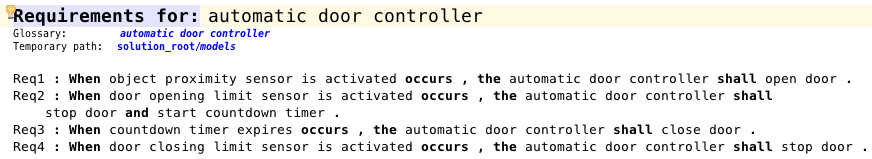
\includegraphics[width=1\textwidth]{images/EARS-Reqs.png}
     \caption{\textsf{EARS-CTRL} Requirements for a sliding door
     controller}
     \label{fig:ears_reqs}
   \end{center} 
 \end{figure}
\vspace{-1cm}Figure~\ref{fig:ears_reqs} illustrates a set of \textsf{EARS-CTRL}
requirements for the software controller for a sliding door. By remaining as close as
possible to the original EARS syntax our editor allows building requirements as
correct English sentences that can easily be written and understood by humans.
In fact, given the requirements stated in figure~\ref{fig:ears_reqs}, no
additional explanations are necessary for a human to understand the behavior of
the sliding door controller that should be generated. In~\cite{LucioRCM17} we
have presented a previous version of \textsf{EARS-CTRL} which included templates
that, although not part of the original EARS, had been introduced to simplify
translation into LTL. In particular we had introduced the possibility of adding
an \emph{until} segment at the end of requirements which is not standard EARS
and which we have removed in the current version of \textsf{EARS-CTRL}.
The work of briging the syntax of \textsf{EARS-CTRL} closer to ``real'' EARS while preserving a semantically
meaniful translation into LTL was done with together with Alistair Mavin, the
author of this paper who is also the main proponent of EARS~\cite{EARS09}.
Our rationale is that, by remaining as faithful as possible to the original EARS
syntax, we: 1) benefit from all the advantages of using EARS already
investigated and described in the literature~\cite{EARS09,EARS16}; and 2)
provide to Rolls-Royce and potentially other companies a tool that can
immediately be used by engineers trained in the use of EARS.\vspace{-.5cm}

\subsection{A Push-Button Approach}

\textsf{EARS-CTRL} can synthesize software controllers directly from EARS
requirements, at the push of a button. Such syntheses are produced 
by the \textsf{autoConf4}~\cite{autoCode17} synthesizer in the form
of a synchronous dataflow (SDF) diagram, which our tool can display
graphically. In the cases where synthesis is not possible the error code from
the \textsf{autoConf4} tool is lifted such that the requirements that prevent
the controller from being generated are pointed out.\vspace{-.5cm} \levi{this is
not done yet}

\subsection{Validation}
\vspace{-.2cm}
% Our \textsf{EARS-CTRL} tool provides a set of mechanisms for verification, in
% particular \emph{Well-Formedness by Construction} when the specification is
% being built and \emph{simulation} of the synthesized controllers by exercising the
% controller manually using \textsf{simulink} as a back-end. We can also generate
% test cases for controllers that can either be used to debug the controller by
% analysing traces of execution of the controller or to be used as test-cases for
% alternative implementations of the controllers which are not automatically
% synthesized.

\subsubsection{Well-Formedness by Construction}
Well-formedness by construction is enforced in two different ways by
\textsf{EARS-CTRL}: firstly, only valid EARS requirement patterns can be added
to a requirements specification. When the requirements engineer picks an EARS
template for her new requirement, the corresponding sentence is displayed by the
IDE as a structure with placeholders. Such structures provide a first level of
well-formedness, as only correctly formed EARS patterns can be added to the
specification. Secondly, only valid sensors or actuators can be picked to fill
in the placeholders in an EARS requirement.\vspace{-.5cm}
\begin{figure}[h!]
   \begin{center}
     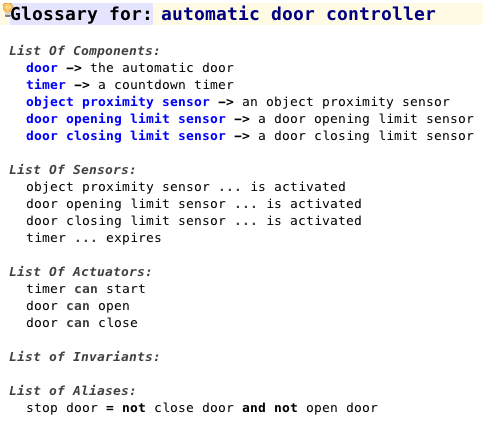
\includegraphics[width=.5\textwidth]{images/glossary.png}
     \caption{\textsf{EARS-CTRL} Glossary for sliding door
     controller}
     \label{fig:ears_glossary}
   \end{center}
 \end{figure} 
\vspace{-1cm}Note that in order to build requirements model illustrated in
figure~\ref{fig:ears_reqs} it is necessary to, as a first step, build a glossary
for the controller. An example of such a glossary is depicted in
figure~\ref{fig:ears_glossary}. The first section of an \textsf{EARS-CTRL}
glossary identifies the components of the system to be controlled. Each one of
those components contains actuators and (possibly) sensors that will be used by
the controller logic as (respectively) inputs from and outputs to the real
system. To allow for more ease of writing when building requirements, aliases
for logical expressions involving sensors or actuators can also be defined in
the glossary. More advanced users also have the possibility of defining
invariant relationships between sensors or actuators.
The vocabulary defined in the glossary is proposed to the requirements engineer
by the \textsf{EARS-CTRL} IDE in order to fill in the placeholders of an EARS
template when a new requirement being written.

Because well-formedness is enforced by construction, requirement specifications
written in \textsf{EARS-CTRL} are always syntactically correct.\vspace{-.4cm} 
\subsubsection{Simulation}
Once a controller has been synthesized from a set of EARS requirements, it
becomes important to understand whether it behaves as expected. In order to do
so we have used the Simulink engine~\cite{simulink} as a simulation back-end.
In figure~\ref{fig:ears_simulator} we display the \textsf{EARS-CTRL} panel that
allows ``playing'' the controller by providing a sequence of inputs manually.
Outputs are incrementally added to the panel as new inputs are provided by the
requirements engineer. Note that, because controllers have internal state,
the order in which the commands influences the controller's output. A ``Reset''
button in the panel allows resetting the controller to its initial
state.
\vspace{-.4cm}
\subsubsection{Generation of Test Cases}
\textsf{EARS-CTRL} allows generating test cases directly from the EARS
requirements. A test case consists of a sequence of $\langle
input, output \rangle$ pairs, where each input is a vector of sensor states
and each output a vector of actuator states. Note that individual sensors and
actuators can assume two states: \textsf{ON} or \textsf{OFF}. Test case
generation is configured by three parameters:\vspace{-.1cm}
\begin{itemize}
  \item \emph{Maximum test case length:} defines the maximum length of the
  $\langle input, output \rangle$ pair sequences to be generated.
  \item \emph{Allow parallel inputs:} enables or disables the possibility of
  having more than one sensor being active for inputs in the test case.
  \item \emph{Allow repeated inputs:} enables or disables having repeated inputs
  in the same test sequence. When enabled this parameter makes it such that
  an input vector cannot occur more than once in a test sequence -- thus
  limiting the length of test sequences to the number of possible input
  vectors.\vspace{-.7cm}
\end{itemize}
\begin{figure}[h!]
   \begin{center}
     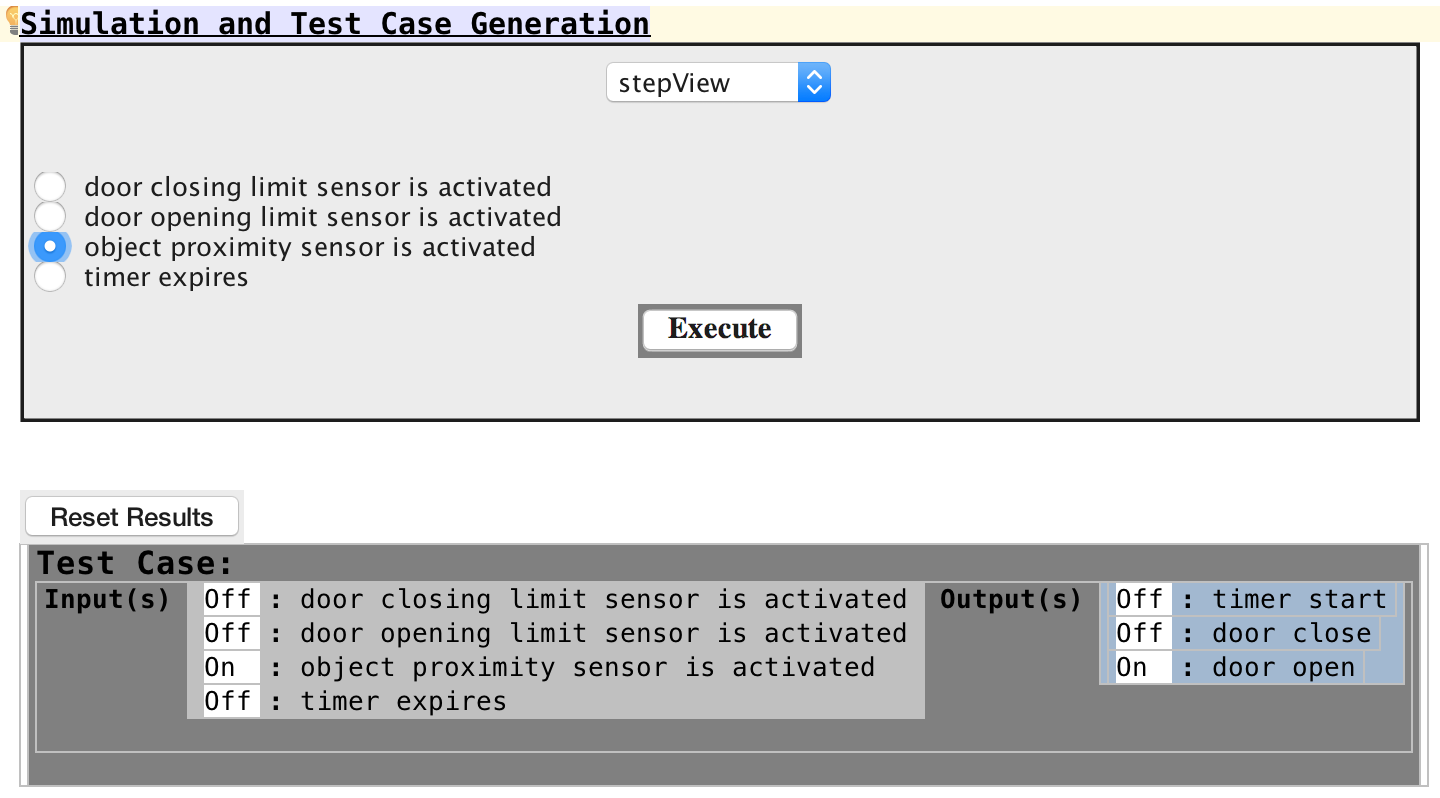
\includegraphics[width=.5\textwidth]{images/simulation.png}
     \caption{\textsf{EARS-CTRL} specification simulator\levi{sync picture
     with text}}
     \label{fig:ears_simulator}
   \end{center}
 \end{figure}
\vspace{-1cm}
Test cases generated by \textsf{EARS-CTRL} can serve two purposes: on
the one hand they are traces of execution of the synthesized controller and can
be used to make sure that controller behaves as expected; on the other hand one
may consider that the synthesizer is not trusted to generate controllers used in
production: in this case the synthesized controller can behave as an oracle to
generate test cases for a production controller implemented using alternative
means.\vspace{-.5cm}
\subsection{Code Generation}
\vspace{-.2cm}Although it is not possible to generate C code for the controller
directly from \textsf{EARS-CTRL}, this can be achieved by directly running Simulink's code
generator on the Simulink model obtained from an \textsf{EARS-CTRL} requirements
specification.


\section{Architecture}

\begin{figure}[t]
   \begin{center}
     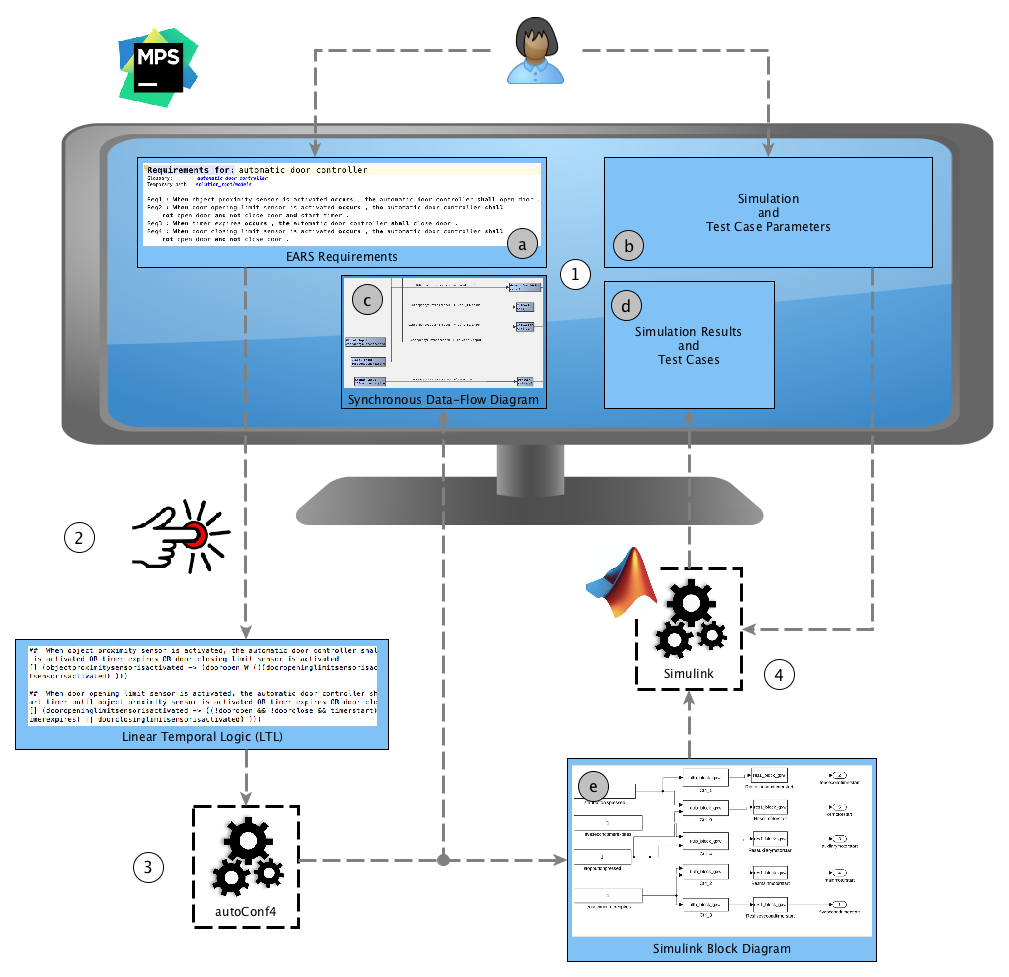
\includegraphics[width=1\textwidth]{images/toolchain.png}
     \caption{The \textsf{EARS-CTRL} Tool Chain\levi{finish pic}}
     \label{fig:ears_ctrl_toolchain}
   \end{center}
 \end{figure}
 
In figure~\ref{fig:ears_ctrl_toolchain} we depict the architecture of the
\textsf{EARS-CTRL} tool. In the following paragraphs we will provide the reader
a brief description of the main components of the tool's architecture, how those
components have been implemented as well as the artifacts they exchange. The
paragraphs are numbered such that each descriptions can be matched with the 
process-related components of the tool depicted in
figure~\ref{fig:ears_ctrl_toolchain}.
Additional letter-labels are used in figure~\ref{fig:ears_ctrl_toolchain} to
refer to data artifacts.
 
\paragraph{1. Editors and Control Panels\\\\} 

The requirements editor, the glossary editor, the simulation and test generation
control panel, the test generation control panel and the synchonous data-flow
diagram visualizer (respectively noted (\textsf{a}), (\textsf{b}), (\textsf{c})
and (\textsf{d}) in figure~\ref{fig:ears_ctrl_toolchain}) have all been built as 
domain-specific languages (DSLs) in the Meta Programming System (MPS) tool. MPS
is both a projectional editor and a domain-specific language workbench.
Domain-specific languages in MPS are composed of an abstract syntax (also known
as meta-model) and a concrete syntax. The concrete syntax allows displaying
and/or editing the information present in a model (as depicted for instance in
figures~\ref{fig:ears_reqs}, \ref{fig:ears_glossary} and
\ref{fig:ears_simulator}). Note that because MPS is a projectional editor, the
abstract syntax is directly edited which avoids an explicit or implicit
intermediate step where the concrete syntax is parsed.
A direct consequence of this is for example the fact that when a component's
name is updated an \textsf{EARS-CTRL} glossary, that update will immediately be
reflected in any requirements that refer to that component name. This automatic
update is an off-the-shelf feature of any editor defined using MPS and is an
easy way to guarantee that references between the several parts of an editor
always remain consistent.

\paragraph{2. From EARS to Lineal Temporal Logic\\\\}
\label{sec:ears_LTL} 

Let us consider the requirement \textsf{Req1} which is part of the
specification of the sliding doors controller in figure~\ref{fig:ears_reqs}:

\begin{center}
\textbf{When} \emph{object proximity sensor is activated} \textbf{then the} \emph{automatic door controller} \textbf{shall}
\emph{open door}.
\end{center}

 This requirement, taken in isolation, translates into the following LTL
 formula:
 
$$[] (objectproximitysensorisactivated \rightarrow dooropen)$$
which, if one takes into consideration the semantics of the $\rightarrow$
operator as ``implies'', is the expected logical meaning of \textsf{Req1}. All EARS
templates, when taken in isolation, can be directly translated into LTL and
propositional logic operators in such a straightforward manner.
If, however, one translates the whole set of requirements for the automatic
door in \ref{fig:ears_reqs} into LTL, the result for \textsf{Req1} will be as follows:

\begin{align*}
[] (object&proximitysensorisactivated \rightarrow\\
 &(dooropen\,W\,(dooropeninglimitsensorisactivated \lor timerexpires\\
 & \lor doorclosinglimitsensorisactivated )))
\end{align*}

This is due to the fact that the requirements specify behaviors that are
interwined during execution. For example, from \textsf{Req1}  in
figure~\ref{fig:ears_reqs} we know that if the \textsf{object proximity sensor}
is activated, the doors will open. We also know from \textsf{Req2} that, when
the \textsf{opening limit reached} sensor is activated, the doors will stop.
Without additional information, the \textsf{autoCode4} synthesis tool identifies
a contradition in these two requirements since, if the two sensors are activated
during the same execution, the doors will logically simultaneously open and
close. In order to avoid such contradictions it becomes necessary to establish a
temporal dependency between the behaviors specified by the requirements. In
order to achieve this our tool performs a static analysis of the requirements
in order to identify such dependencies and to add this information to the
generated LTL specification.
This additional contextual information in the generated LTL is clear from the
second translation above:
the door will only open, \emph{until} (the ``\textbf{W}'' operator) the door \textsf{opening limit
reached} sensor is activated, \emph{or} other events stated in related
requirements occur.
 
\paragraph{3. Synthesizing a Controller using \textsf{autoCode4}\\\\}
 
Controller synthesis is achieved via \textsf{autoCode4}'s Java API. The LTL
specification obtained as explained in section~\ref{sec:ears_LTL} is passed into
the synthesizer which returns a synchronous data-flow (SDF) diagram as an Java
object instance. The SDF diagram is then parsed and rebuilt as a visual model
which is an instance of the synchonous data-flow diagram visualizer DSL
(identified by label (\textsf{e}) in figure~\ref{fig:ears_reqs}). Such a visual
model provides the requirements engineer with a graphical and technical view of
the synthesized controller as a set of blocks and wires which can be used as a
debugging artifact.

\paragraph{4. Simulation and Test Generation using Simulink\\\\}

The SDF diagram obtained from the \textsf{autoCode4}
consists, for short, of a set of synchronized blocks that perform arithmetic,
logical or other functions on input signals and return the result on output signals. The controller's inputs and
outputs are also themselves represented as blocks. The fashion in which blocks
are synchronized is declared by connecting those blocks' inputs and outputs via
wires. In order to simulate \textsf{EARS-CTRL} specifications we have built a
translator from such data-flow diagrams onto Simulink models. Given that the SDF
formalism is very similar to the Simulink formalism, the structural translation
is essentially one-to-one. However, only a subset of all blocks present in
the SDF specifications that are produced by \textsf{autoCode4} is available
off-the-shelf in Simulink. As such, a number of Simulink blocks had to be built
by us to accommodate the semantics of SDF specifications. In
particular we had to build a number of stateful blocks to mimic in Simulink the
operation of some of SDF's blocks.

The Simulink model is generated by \textsf{EARS-CTRL} as a Mathlab simulink
script that builds the model programmatically (label \textsf{e} in
figure~\ref{fig:ears_reqs}). Communication with simulink from the \textsf{EARS-CTRL} IDE for
simulation and test case generation is also programatically achieved through the
use of the \textsf{mathlabcontrol}\cite{mathlabcontrol} Java API.


\section{Related Work}

Given the recent fast-paced development of Artificial Intelligence relying
on increasigly powerful hardware, a number of projects have devoted effort to the
generation of controllers from requirements. The ARSENAL
project~\cite{ghosh2016arsenal} has as starting point specifications written in
arbitrary natural language and uses the GR-1~\cite{piterman2006synthesis}
synthesizer for automatically building controllers. In~\cite{YanCC15} the
authors also use the GR-1 synthesizer to automatically build robot
controllers. The work of Yan et. al.~\cite{YanCC15} takes as inputs full LTL
specifications and includes features such as the use of dictionaries for
automatically derive relations between terms, or guessing the I/O partitioning
that allow detecting inconsistencies in the specifications. The commercial
argosym STIMULUS tool~\cite{jeannet16}, while not based on AI algorithms from controller
synthesis, is a commercial platform that allows specifying requirements in a
formal language using a close-to natural language syntax. Requirements expressed
in STIMULUS can be simulated in order to look for inconsistencies and test
cases can also be directly generated from the requirements. 

Our approach differs from the GR-1-based projects mentioned above in the sense
that we do not aim at applying pure natural language parsing to arbitrary
requirements. Using EARS allows us to provide the readability of the English
language while gently contraining it to fit the domain of requirements
gathering. Also, rather than using the full expressiveness of LTL, we have
restricted our approach to the \textsf{GXW} subset of LTL which is handled by
the \textsf{autoCode4} tool. Using this subset it is possible to directly
generate controllers as SDF diagrams, which are easy to inspect and to simulate.
Tools that are based on GR-1 or bounded synthesis~\cite{schewe2007bounded}
typically produce controllers as BDD or explicit state machine structures that
can be very large and difficult to inspect or simulate.

Regarding the STIMULUS tool, our approach was conceptually though of starting
from an opposite direction -- while STIMULUS essencially uses as central
formalism state machines wrapped by a syntactic-sugar English-like specification
language, \textsf{EARS-CTRL} uses a constrained version of the English language.
We have purposefully placed EARS at the center on our tool -- the goal has been
to adapt the subset of LTL used by \textsf{autoCode4} to EARS and to remain
unbiased towards the formalisms ``under the hood''. Unlike in our work, STIMULUS
relies on the state machines underlying the requirements to allow simulation as
in fact the approach's goal is to verify requirements and not to synthesize
usable controllers.



\section{Limitations and Future Work}
\label{sec:limfuturework}

Due to the boolean representation of sensors and actuators in \textsf{autoConf4}
 it is currently not possible for \textsf{EARS-CTRL} to express or analyze
states of the system that involve numerical data. This naturally limits our
approach to controllers for systems where sensors or actuators can be
represented using boolean types.
For instance, expressing a state such as ``the throttle is pushed to 1/4 of its
capacity'' using \textsf{EARS-CTRL} would at best involve modelling four
different sensors in order to partition the input space of a single sensor. Such
an approach may prove to be infeasible and/or impractical in the real world and
other code synthesizers for \textsf{EARS-CTRL}  might be considered in the
future.\levi{which ones?}

Future work will concentrate on exploring the usability of
\textsf{EARS-CTRL} for larger case studies. In particular we expect to continue
the collaboration with Rolls-Royce in order obtain real requirements such that
the synthesis and verification mechanisms explained in this paper can be put to
the test in the field. It of particular interest to understand not only how
\textsf{EARS-CTRL} \textsf{autoConf4} based-synthesis will scale, but also to
which extent the verification and debug mechanisms we propose are helpful in
practice.\levi{is this too self-deprecating?}


\section{Conclusions and Future Work}

%
% ---- Bibliography ----
%
\bibliographystyle{abbrv}
\bibliography{models_tool_2017}

\end{document}
